\documentclass{article}
\usepackage{graphicx} % Requerido para insertar imagenes
\graphicspath{ {img/} }
\usepackage[square,numbers]{natbib}
\usepackage[spanish]{babel}
\usepackage{amsmath}
\usepackage{float}



\title{Artículo}
\author{Sonia Torres Ibarra}
\date{\today}


\begin{document}

\maketitle

\section{Introducción}

En el análisis de datos, los algoritmos no supervisados juegan un papel fundamental al permitir descubrir estructuras subyacentes sin necesidad de etiquetas o clases predefinidas. Estos métodos son ampliamente utilizados en contextos donde se busca identificar patrones, segmentar observaciones o reducir la complejidad de los datos, como en la exploración de clientes, análisis de comportamiento o clasificación automática de información.\\

Entre las técnicas más comunes se encuentran los algoritmos de clustering, que agrupan elementos con características similares. Sin embargo, la elección del algoritmo adecuado depende tanto de la naturaleza de los datos como de la forma en que se desea representar la similitud entre observaciones. En este trabajo se investigó una alternativa adicional a los métodos vistos en clase, considerando el modelo DBSCAN, el cual ofrece ventajas frente a algoritmos clásicos como k-means, especialmente cuando los datos presentan ruido, densidades variables o formas de agrupamiento no esféricas.\\

Para evaluar la calidad de los grupos obtenidos, se consideran métricas como el Silhouette Score y el índice Davies-Bouldin, que permiten cuantificar de manera objetiva la representatividad de las segmentaciones. Este enfoque busca no solo identificar patrones significativos, sino también respaldar los resultados mediante criterios matemáticos claros.\\

De manera complementaria, se aborda el aprendizaje supervisado mediante el modelo de regresión lineal, con el fin de predecir variables de interés a partir de un conjunto de predictores. La efectividad de estas predicciones se evalúa mediante métricas, como el Error Absoluto Medio (MAE) y la Raíz del Error Cuadrático Medio (RMSE), proporcionando una medida cuantitativa de la precisión del modelo.\\

En conjunto, el trabajo presenta la aplicación práctica de técnicas supervisadas y no supervisadas sobre un conjunto de datos reales, acompañado del análisis de resultados, la interpretación de las métricas utilizadas y la referencia a investigaciones previas que respaldan la metodología implementada.
\clearpage
\section{Descripción de los datos}

La Comisión Nacional Bancaria y de Valores (CNBV), en colaboración con el Instituto Nacional de Estadística y Geografía (INEGI), realizaron la Encuesta Nacional de Inclusión Financiera (ENIF) 2024. Su objetivo es generar información estadística e indicadores oficiales a nivel nacional que permitan a las autoridades financieras hacer diagnósticos, diseñar políticas públicas y establecer metas en materia de inclusión y educación financieras. Asimismo, incorporar cambios y actualizaciones para dar atención a nuevos requerimientos de información y consideraciones en la Política Nacional de Inclusión Financiera (PNIF).


\section{Antecedentes}

Investigaciones relacionadas:\\

El autor Cando \cite{candofacultad} menciona que "DBSCAN, se distingue por su capacidad para identificar agrupaciones de formas irregulares y destacar puntos de datos aislados como outliers, lo
que lo convierte en una herramienta valiosa para discernir comportamientos financieros
altamente atípicos entre los socios" .

\section{Metodología}

\subsection{Aprendizaje no supervisado}
El DBSCAN es un algoritmo no supervisado muy conocido en materia de Clustering. Fue presentado en 1996 por Martin Ester, Hans-Peter Kriegel, Jörg Sander y Xiawei Xu.\cite{ml_dbscan_ds}\\

El algoritmo DBSCAN identifica grupos de datos (clústeres) mediante la estimación de densidades locales en el espacio de observaciones. Su funcionamiento puede resumirse en cuatro etapas principales:
\begin{itemize}
  \item Para cada observación miramos el número de puntos a una distancia máxima $\epsilon$ de ella. Esta zona se denomina $\epsilon$-vecindad de la observación.
  \item Si una observación tiene al menos un cierto número de vecinos, incluida ella misma, se considera una observación central. En este caso, se ha detectado una observación de alta densidad.
  \item Todas las observaciones en la vecindad de una observación central pertenecen al mismo clúster. Puede haber observaciones centrales cercanas entre sí. Por lo tanto, de un paso a otro, se obtiene una larga secuencia de observaciones centrales que constituyen un único clúster.
  \item Cualquier observación que no sea una observación central y que no tenga ninguna observación central en su vecindad se considera una anomalía.
\end{itemize}

DBSCAN por lo general utiliza la distancia euclidiana\\

\begin{math}
d(p,q)=\sqrt{(p_1-q_1)^2+(p_2-q_2)^2+...+(p_i-q_i)^2+...+(p_n-q_n)^2}=\sqrt{\sum_{i=1}^{n} (p_i-q_i)^2}
\end{math}\\

En cada observación, para contar el número de vecinos a como máximo una distancia $\epsilon$, calculamos la distancia euclidiana entre el vecino y la observación y comprobamos si es inferior a $\epsilon$.

DBSCAN utiliza dos parámetros principales \cite{datacamp}:
\begin{itemize}
    \item eps (épsilon): La distancia máxima entre dos puntos para que se consideren vecinos.
    \item min samples: El número mínimo de puntos necesarios para formar una región densa.
\end{itemize}

Por lo tanto, antes de aplicar DBSCAN es indispensable definir dos parámetros clave que determinan la estructura final del agrupamiento:
\begin{itemize}
\item ¿Qué distancia $\epsilon$ hay que determinar para cada observación la $\epsilon$-vecindad? 
\item ¿Cuál es el número mínimo de vecinos necesario para considerar una observación como una observación central?
\end{itemize}


En este trabajo, para seleccionar los parámetros óptimos del algoritmo DBSCAN , se utilizaron métricas internas de validación de clustering, específicamente el Silhouette Score y el Davies-Bouldin Index.\\

El índice Silhouette\cite{silhoutte}  evalúa simultáneamente la cohesión interna (qué tan cerca están los puntos dentro de un mismo clúster) y la separación externa (qué tan distintos son los clústeres entre sí). Para cada punto $i$, se calcula la distancia promedio a los demás puntos de su propio clúster ($a_i$) y la distancia promedio al clúster más cercano ($b_i$). Su valor se obtiene mediante:

\begin{math}
s_i=\frac{b_i-a_i}{max(a_i,b_i)} \
\end{math}\\

con rango [−1,1], donde valores cercanos a 1 indican clusters bien definidos y separados, valores cercanos a 0 indican puntos en los límites de los clusters, y valores negativos sugieren posible asignación incorrecta \cite{scikitlearn_clustering}.

El coeficiente de la Silhouette ($s_i$) se define para cada clúster. Cuando se dispone de más de dos clústeres se calcula el valor promedio de la Silhouette para disponer de una medida de la calidad de los clústeres.\\

Por otro lado, el Davies-Bouldin Index (DBI) \cite{Davies_Bouldinen} se basa en relacionar la dispersión dentro de los clústeres (intra-clúster) y la separación entre clústeres (inter-clúster). Por un lado, la dispersión intra-clúster mide la separación de los puntos dentro de cada clúster. Una dispersión intra-clúster baja indica que los puntos dentro de un grupo están muy cercanos entre sí, algo que es deseable en un buen clustering. Por otro lado, la dispersión inter-clúster mide la separación entre los grupos. Una dispersión inter-clúster alta indica que los grupos están muy alejados entre sí, lo que también es deseable en un buen clustering. El índice de Davies-Bouldin se construye como el cociente de ambos valores. Por lo que cuando los clústeres están separados y son compactos el valor de este índice se minimiza.:

\begin{math}
DB=\frac{1}{k} \sum_{i=1}^{k} \max_{j \neq i} \frac{S_i+S_j}{M_{ij}} \\
\end{math}

donde $S_i$ es la dispersión promedio dentro del cluster $i$ y $M_{ij}$ la distancia entre los centroides de los clusters $i$ y $j$. Valores bajos de DBI indican clusters más compactos y mejor separados.

Para aplicar estas métricas, se probó DBSCAN con distintas combinaciones de eps y min samples, calculando Silhouette y Davies-Bouldin para los clusters detectados (excluyendo outliers). La combinación que maximizó el Silhouette Score y minimizó el Davies-Bouldin Index fue seleccionada como óptima, asegurando así una segmentación más representativa y coherente de los datos.

\subsection{Aprendizaje supervisado: Regresión lineal}

La regresión lineal es un método estadístico que trata de modelar la relación entre una variable continua y una o más variables independientes mediante el ajuste de una ecuación lineal. Se llama regresión lineal simple cuando solo hay una variable independiente y regresión lineal múltiple cuando hay más de una. Dependiendo del contexto, a la variable modelada se le conoce como variable dependiente o variable respuesta, y a las variables independientes como regresores, predictores o features.\cite{ciencia_datos_net}  \\

El modelo de regresión lineal considera que, dado un conjunto de observaciones 
${\{y_i,x_{i1},...,x_{np}\}_{i=1}^{n}$ la media $\mu$ de la variable respuesta y se relaciona de forma lineal con la o las variables regresoras $x_i$...$x_p$, acorde a la ecuación:

\begin{math}
\mu_y= \beta_0 + \beta_1 x_1+ \beta_2 x_2+...+ \beta_p x_p\\
\end{math}

La interpretación de los elementos del modelo:

\begin{itemize}
\item  $\beta_0$ es la ordenada en el origen, se corresponde con el valor promedio de la variable respuesta y cuando todos los predictores son cero.
\item $\beta_p$ es el efecto promedio que tiene sobre la variable respuesta el incremento en una unidad de la variable predictora $x_p$
\end{itemize}

En la gran mayoría de casos, los valores $\beta_0$ y $\beta_p$ poblacionales son desconocidos, por lo que, a partir de una muestra, se obtienen sus estimaciones 
$\hat{\beta_0}$ y $\hat{\beta_p}$.
Ajustar el modelo consiste en estimar estos coeficientes de forma que se minimicen los errores de predicción, es decir, que la línea ajustada represente de la mejor manera la tendencia de los datos observados.

El método empleado con más frecuencia es el ajuste por mínimos cuadrados ordinarios (OLS), que identifica como mejor modelo la recta (o plano si es regresión múltiple) que minimiza la suma de las desviaciones verticales entre cada dato de entrenamiento y la recta, elevadas al cuadrado.\\

Estos cálculos son más eficientes si se realizan de forma matricial\cite{datacamp_LR}:

\begin{math}
\beta= (X^TX)^{-1}X^Ty
\end{math}

Dónde:
\begin{itemize}
\item $X$ es la matriz de variables independientes (con una columna de unos para el intercepto),
\item $y$ es el vector de valores de la variable dependiente.
\item $X^T$ es la transposición de la matriz de $X$.
\item $(X^TX)^{-1}$ es la inversa de $X^TX$.
\end{itemize}

Esta ecuación da los valores óptimos de los coeficientes que minimizan la suma de errores al cuadrado.\\

Para evaluar la calidad del ajuste y cuantificar los errores del modelo, se utilizaron las métricas: coeficiente de determinación $R^2$ ,  MAE (Mean Absolute Error en español error absoluto medio) y RMSE (Root Mean Squared Error Root Mean Squared Error en español raíz del error cuadrático medio). Estas permiten medir el grado de precisión y consistencia del modelo de regresión al comparar los valores predichos con los observados.\\

El coeficiente de determinación ($R^2$) mide la precisión con la que un modelo estadístico predice un resultado \cite{coef_determinacion}. El valor más bajo posible de $R^2$ es 0 y el valor más alto posible es 1. En pocas palabras, cuanto mejor sea un modelo para hacer predicciones, más cerca estará su $R^2$ de 1.


\begin{math}
R^2=1-\frac{\sum_{i=1}^{n} (y_i-\hat{y_i})^2}{\sum_{i=1}^{n} (y_i-\bar{y_i})^2}  \\
\end{math}

El nominador mide la distancia entre los valores reales y los valores predecidos por el modelo al cuadrado, es decir, es la suma del error al cuadrado. El denominador es la variación total en los datos observados, nos indica cuánto se alejan los valores reales de la media (promedio) de la variable dependiente.\\

El MAE\cite{mae_datacamp} mide la magnitud promedio de los errores en un conjunto de predicciones, sin considerar su dirección. Es el promedio de las diferencias absolutas entre los valores predichos y los reales.

\begin{math}
MAE=\frac{1}{n}\sum_{i=1}^{n} \left|y_i-\hat{y}_i\right| \\
\end{math}

El MAE resulta útil cuando se busca una interpretación directa del error promedio sin dar un peso excesivo a los errores grandes. Es especialmente apropiado en contextos donde existen valores atípicos o cuando no se desea penalizar de forma desproporcionada las desviaciones extremas.\\

El RMSE\cite{rmse_datacamp} es la raíz cuadrada de la media de las diferencias al cuadrado entre los valores observados y los predichos. Es una métrica de regresión muy utilizada que nos indica cuánto error debemos esperar de nuestras predicciones, por término medio. 

\begin{math}
RMSE=\sqrt{\frac{1}{n} \sum_{i=1}^{n} \left( y_i - \hat{y}_i \right)^2} \\
\end{math}

Al elevar al cuadrado los residuos antes de promediarlos, el RMSE penaliza más los errores grandes que los pequeños. Esta sensibilidad hace que sea una buena elección cuando no se desean grandes errores de predicción. El RMSE siempre es no negativo, y los valores más bajos indican un modelo mejor ajustado.\\

La biblioteca scikit-learn facilita la aplicación de la regresión lineal:
\begin{itemize}
\item Tiene una interfaz coherente. El código necesario para aplicar los distintos algoritmos de ML es similar.
\item El código es sencillo, y se han eliminado los complejos detalles matemáticos y de implementación. Por ejemplo, para ajustar un modelo a los datos de entrenamiento, basta con utilizar la línea model.fit(\texttt{X\_train}, \texttt{y\_train}).
\item Facilita el acceso a los coeficientes del modelo.
\item Proporciona métricas integradas para evaluar el rendimiento del modelo.
\item Es fácil integrar la regresión lineal (o cualquier otro algoritmo de ML) con pasos de preprocesamiento, como el escalado y la selección de características, utilizando Pipeline.
\end{itemize}



\section{Resultados}

\subsection{Aprendizaje no supervisado}
En la figura 1 (p.\pageref{fig:resultado}) se muestran los resultados de aplicar DBSCAN sobre los datos, evaluando distintos valores de los parámetros eps y min samples. Se incluyeron métricas de validación  como Silhouette Score y Davies-Bouldin Index para determinar la calidad de los clusters obtenidos y los parámetros a utilizar.

\begin{figure}[H]
    \centering
    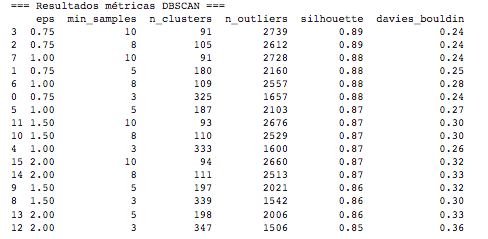
\includegraphics[width=1\linewidth]{Resultado_1.png}
    \caption{Resultados para pruebas DBI y Silhouette}
    \label{fig:resultado}
\end{figure}

El valor más alto de Silhouette (0.89) se obtiene para eps=0.75 y min samples=10. Esto sugiere que los clusters detectados bajo estos parámetros presentan una buena separación relativa entre ellos.\\

Para el índice de Davies-Bouldin, los valores más bajos  se observan también en los parámetros de eps=0.75 y min samples 8-10, corroborando la cohesión detectada por Silhouette.\\

Considerando ambas métricas, los parámetros eps=0.75 y min samples=10 fueron seleccionados como los más adecuados, ya que logran un balance entre número razonable de clusters y alta calidad de agrupamiento.\\

DBSCAN, con eps=0.75 y min samples=10, detecta 91 grupos principales de usuarios y destaca la heterogeneidad mediante la gran cantidad de outliers.

\begin{figure}[H]
    \centering
    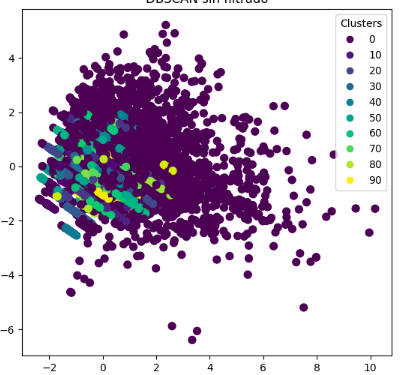
\includegraphics[width=0.5\linewidth]{Resultado_2.png}
    \caption{Gráfico DBSCAN con los parámetros seleccionados.}
    \label{fig:dbscan:graphic}
\end{figure}


\begin{table}
\caption{Clusters obtenidos}
\centering
\begin{tabular}{|l|r|} \hline 
Cluster & Casos \\ \hline \hline
-1      & 2739  \\ \hline
0       & 13   \\ \hline
1     & 337  \\ \hline
--       & --    \\ \hline
90     & 10    \\ \hline
\end{tabular}
\label{tab:clusters}
\end{table}


\subsection{Aprendizaje supervisado: Regresión lineal}

Para efectos de aplicar un modelo de pronóstico, se estimó la variable continua \textit{ingreso}, aplicando un modelo de regresión lineal. Este enfoque permitió evaluar la relación entre el ingreso y los distintos factores explicativos, así como generar predicciones  sobre los valores de la variable ingreso. \\

El resultado obtenido fue:

\textbf{$
ingreso\_mensual = 2448.63 + 825.47*nivel\_estudio + 1062.40*frecuencia\_ingreso + 862.30*uso\_app\_medir\_gastos + 577.93*curso\_ef + 8265.77*tiene\_cuenta\_cheques + 170.37*tiene\_cuenta\_ahorro + 4828.70*tiene\_fondo\_inv + 1152.50*guardo\_dinero\_en\_cualquier\_cuenta + 231.19*tiene\_tdc\_departamental + 319.42*tiene\_prestamo\_nomina + 33.22*tiene\_prestamo\_personal + 6824.62*tiene\_credito\_automotriz + 2129.35*tiene\_credito\_vivienda - 1703.50*tiene\_credito\_grupal - 360.81*tiene\_credito\_apps + 3136.19*tiene\_tdc\_credito$}\\

Los resultados obtenidos se evaluaron mediante métricas de calidad de ajuste y cuantificación de errores como el coeficiente de determinación ($R^2$), el error absoluto medio (MAE) y la raíz del error cuadrático medio (RMSE), con el fin de analizar la precisión y consistencia del modelo.\\

El modelo presentó un coeficiente de determinación $R^2 = 0.310$, indicando que aproximadamente el 31\% de la variabilidad observada en la variable ingreso fue explicada por las variables predictoras consideradas. La magnitud promedio de los errores de predicción, medida mediante MAE, fue de 5,201.13 pesos, mientras que el RMSE alcanzó 8,305.77 pesos, reflejando la penalización de los errores grandes y proporcionando una medida de la dispersión de los residuos.\\

Los coeficientes estimados del modelo de regresión se presentan en la Tabla~\ref{tab:coef_regresion}, mostrando la contribución de cada variable predictora sobre el ingreso:

\begin{table}[h!]
\centering
\caption{Coeficientes del modelo de regresión lineal para la predicción del ingreso}
\label{tab:coef_regresion}
\begin{tabular}{l r}
\hline
\textbf{Variable} & \textbf{Coeficiente} \\
\hline
nivel\_estudio & 825.47 \\
frecuencia\_ingreso & 1,062.40 \\
uso\_app\_medir\_gastos & 862.30 \\
curso\_ef & 577.93 \\
tiene\_cuenta\_cheques & 8,265.77 \\
tiene\_cuenta\_ahorro & 170.37 \\
tiene\_fondo\_inv & 4,828.70 \\
guardo\_dinero\_en\_cualquier\_cuenta & 1,152.50 \\
tiene\_tdc\_departamental & 231.19 \\
tiene\_prestamo\_nomina & 319.42 \\
tiene\_prestamo\_personal & 33.22 \\
tiene\_credito\_automotriz & 6,824.62 \\
tiene\_credito\_vivienda & 2,129.35 \\
tiene\_credito\_grupal & -1,703.50 \\
tiene\_credito\_apps & -360.81 \\
tiene\_tdc\_credito & 3,136.19 \\
\hline
\end{tabular}
\end{table}

Del análisis de los coeficientes, se observa que algunas variables tienen un efecto positivo notable sobre el ingreso, como \textit{tiene\_cuenta\_cheques}, \textit{tiene\_fondo\_inv} y \textit{tiene\_credito\_automotriz}, mientras que ciertas variables presentan efectos negativos, como \textit{tiene\_credito\_grupal} y \textit{tiene\_credito\_apps}. Estas relaciones reflejan cómo diferentes aspectos del comportamiento financiero y del acceso a servicios bancarios influyen en los niveles de ingreso de los encuestados.\\

En conjunto, las métricas de desempeño y los coeficientes estimados permiten concluir que, aunque el modelo explica una fracción importante de la variabilidad del ingreso, aún existe dispersión no capturada, sugiriendo que factores adicionales podrían mejorar la predicción.


\section{Conclusiones y discusión}

Esta tarea permitió explorar dos enfoques del aprendizaje automático: supervisado y no supervisado.\\

En el enfoque no supervisado se aplicó el algoritmo DBSCAN como una alternativa para la detección de patrones y agrupamientos. A diferencia de otros métodos más rígidos, como k-means, DBSCAN no requiere definir previamente el número de grupos.


La selección de parámetros se realizo con el índice de Silhouette y el índice de Davies-Bouldin. Estos indices permitieron analizar la relación interna de los clústeres y la separación entre ellos, proporcionando una visión más completa del desempeño del modelo. Los valores reflejaron una estructura de clústeres bien definida y con baja superposición entre grupos. Sin embargo, se identificó una cantidad considerable de outliers, lo que sugiere la existencia de observaciones atípicas o de baja densidad en los datos.

Los hallazgos confirman que DBSCAN es un buen algoritmo para la identificación de patrones en datos complejos, siempre que se realice una selección cuidadosa de sus parámetros y se complementen los resultados con métricas de validación adecuadas. \\

Por su parte, el modelo de regresión lineal permitió estimar la variable continua \textit{ingreso}, identificando cómo diferentes factores financieros influyen en los niveles de ingreso de los encuestados. Las métricas de desempeño del modelo, como $R^2$, MAE y RMSE, ayudaron a evaluar la precisión de las predicciones, mientras que los coeficientes estimados mostraron qué variables tienen un impacto positivo o negativo sobre el ingreso.  

\bibliographystyle{abbrvnat}
\bibliography{biblio}


\end{document}








